\documentclass[12pt,a4paper]{article}

% Packages
\usepackage[utf8]{inputenc}
\usepackage{geometry}
\usepackage{graphicx}
\usepackage{booktabs}
\usepackage{hyperref}
\usepackage{listings}
\usepackage{xcolor}
\usepackage{float}
\usepackage{caption}
\usepackage{subcaption}
\usepackage{enumitem}
\usepackage{titlesec}
\usepackage{amsmath}
\usepackage{algorithm}
\usepackage{algpseudocode}

\geometry{margin=0.72in}
\setlength{\parindent}{0pt}
\setlength{\parskip}{0.42em}
\linespread{0.98}
\setlength{\emergencystretch}{2em}
\setlist[itemize]{leftmargin=*, itemsep=0.2em, topsep=0.35em, parsep=0em, partopsep=0em}
\setlist[enumerate]{leftmargin=*, itemsep=0.2em, topsep=0.35em, parsep=0em, partopsep=0em}
\titlespacing*{\section}{0pt}{1.3ex plus 0.2ex minus 0.2ex}{0.7ex plus 0.2ex}
\titlespacing*{\subsection}{0pt}{1.1ex plus 0.2ex minus 0.2ex}{0.5ex plus 0.2ex}
\titlespacing*{\subsubsection}{0pt}{0.9ex plus 0.2ex minus 0.2ex}{0.4ex plus 0.15ex}
\captionsetup{font=small}
\urlstyle{same}
\setcounter{tocdepth}{2}

% Code listing style
\lstset{
    basicstyle=\ttfamily\footnotesize,
    breaklines=true,
    frame=single,
    backgroundcolor=\color{gray!10},
    keywordstyle=\color{blue},
    commentstyle=\color{green!50!black},
    stringstyle=\color{orange}
}

\newcommand{\runname}[1]{\texttt{\detokenize{#1}}}
\newcommand{\command}[1]{\texttt{\detokenize{#1}}}
\newcommand{\fpath}[1]{\texttt{\detokenize{#1}}}

% Title information
\title{%
    \textbf{Viability of Synthetic-Data-Only Training for Vehicle Detection}\\
    \large A Study on Real-World Performance, Run Management, and Gemini API Scaling
}
\author{%
    Esad Kaya\\
    Student Number: 300283659\\
    \texttt{ekaya@uOttawa.ca}
}
\date{%
    \today\\[1em]
    \normalsize SEG 4180: Applied Machine Learning\\
    Professor Daniel Shapiro\\
    University of Ottawa
}

\begin{document}

\pagenumbering{gobble}
\maketitle
\thispagestyle{empty}

\begin{abstract}
	This report evaluates whether a high-performing vehicle detector can be trained using synthetic data only. The project built a full run-scoped pipeline around Google Street View backgrounds, Gemini image editing, auto-label generation, manual review, leakage-safe group splitting, and YOLO11 training. The strongest model came from the folded configuration in \fpath{runs/Combined_Run_004_Folded/}, where the former \fpath{lookalike_negative} category was absorbed into the main vehicle class. That final YOLO11n run achieved precision 0.976, recall 0.946, mAP@0.5 of 0.973, and mAP@0.5:0.95 of 0.939 on real-world imagery. The technical conclusion is positive: synthetic-only training worked. The practical conclusion is more mixed: the approach required careful scene gating, disciplined experiment isolation, and much stricter API-cost control than initially expected.
\end{abstract}

\newpage
\pagenumbering{roman}
\tableofcontents

\newpage
\pagenumbering{arabic}

%=============================================================================
\section{Introduction}
%=============================================================================

\subsection{Motivation}

The central question of this project was whether synthetic data alone could support a practically useful multi-class vehicle detector for street-level imagery. The target use case focused on rare enforcement vehicles, including Ottawa police liveries, where organic collection is slow, class-imbalanced, expensive, and operationally awkward. Rather than waiting for rare examples to appear naturally, the pipeline inserts controlled vehicle variants into realistic empty road scenes and then trains YOLO11 on the resulting labeled dataset.

The problem is not only model accuracy; it is pipeline credibility. A synthetic-only workflow must solve four issues at once: scene selection, visual realism, label quality, and leakage-safe evaluation. This report therefore treats the model as the end product of a larger system rather than an isolated training script.

\subsection{Project Context and Preprocessing}

Google Street View images include a logo strip and occasional stitching artifacts along the bottom edge. Those patterns should not become learned shortcuts during training or inference. A dedicated crop stage, implemented in \fpath{scripts/02b_crop_bottom.py}, removes the bottom 30 pixels from each image. The crop amount was selected empirically because it consistently removes the Google branding while preserving nearby vehicle content. The script is idempotent, so reruns do not repeatedly degrade the same assets.

This preprocessing detail matters because the project aimed for a consistent train--validation--inference path. If cropping is applied during training but not during deployment, the detector sees a different input distribution and performance degrades. The pipeline therefore treats the crop as a first-class preprocessing contract, not an ad hoc cleanup step.

%=============================================================================
\section{Empty Frame Detection and Scene Gating}
%=============================================================================

\subsection{Overview}

Synthetic insertion starts with negative backgrounds: frames that contain no vehicles and still depict a plausible roadway scene. The empty-frame stage is therefore the main quality gate before any expensive generation calls are made.

\subsection{Method}

The pipeline applies a two-stage filter. First, a COCO-pretrained YOLO model scans all frames with a deliberately low confidence threshold in the 0.15--0.25 range to minimize false negatives. Second, Gemini evaluates whether the candidate image is a valid street or road scene. Instead of silently discarding borderline cases, the pipeline writes traceable outputs and list files. The two primary artifacts are \fpath{lists/empty_candidates.txt}, which records all frames deemed vehicle-free, and \fpath{lists/valid_road_candidates.txt}, which records the subset that also passes the road-scene gate.

This design improved quality in two ways. It prevented synthetic edits from being applied to sidewalks, alleys, interiors, and other visually implausible contexts, and it reduced the amount of downstream manual review required in the labeler. Operationally, it also provided a more cost-effective alternative to manual collection of thousands of real photographs in the hope of capturing enough rare enforcement vehicles.

%=============================================================================
\section{Synthetic Data Generation}
%=============================================================================

\subsection{Overview}

The core generation stage inserts vehicles into empty Street View frames using generative AI. This gives the project direct control over class balance and makes it possible to generate rare enforcement categories at will. In practice, each base frame can produce a random vehicle variant, an enforcement vehicle variant, and police variants corresponding to older and newer Ottawa liveries.

\subsection{Synthesis Statistics}

Table~\ref{tab:run_composition} summarizes the major dataset configurations used across the project. The important point is that later runs were not merely new model settings; they also reflected different data mixes and run-management practices.

\begin{table}[H]
	\centering
	\begin{tabular}{lrrr}
		\toprule
		\textbf{Run}            & \textbf{Original} & \textbf{Synthetic} & \textbf{Total} \\
		\midrule
		Legacy Root Run 001     & 9,600             & 2,581              & 12,181         \\
		Benchmark Run 002       & 3,203             & 4,209              & 7,412          \\
		Combined Run 003        & 3,203             & 6,784              & 9,987          \\
		Combined Run 004 Folded & 3,203             & 6,784              & 9,987          \\
		\bottomrule
	\end{tabular}
	\caption{Per-run image composition. The legacy run used the original Street View collection, while later runs used a more curated base pool after scene gating.}
	\label{tab:run_composition}
\end{table}

The run totals matter when interpreting training outcomes. The legacy run used 12,181 images, the benchmark run used 7,412, and both combined runs used 9,987. The later combined runs therefore traded raw breadth of original imagery for a denser and more intentional synthetic mix.

Figure~\ref{fig:synth_examples} shows synthetic vehicle examples.

\begin{figure}[H]
	\centering
	\fbox{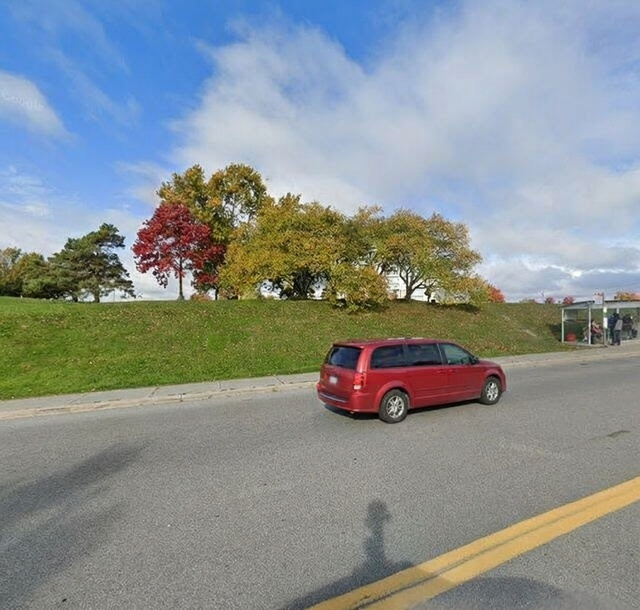
\includegraphics[width=0.35\textwidth]{synthetic-random-vehicle.jpg}}
	\fbox{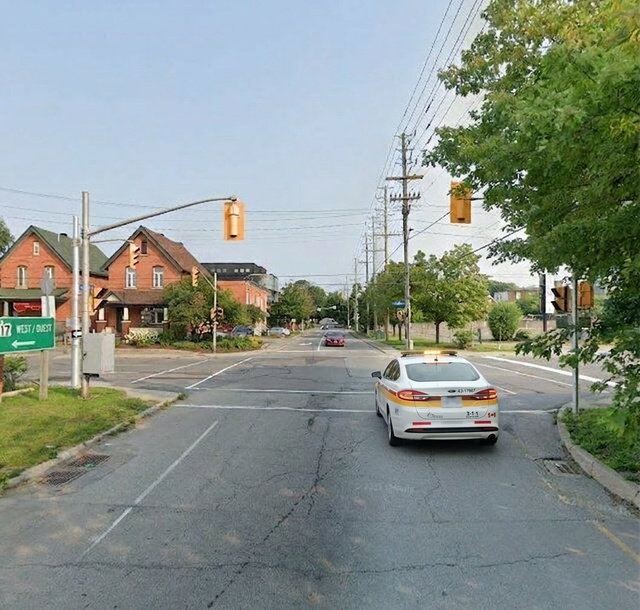
\includegraphics[width=0.35\textwidth]{synthetic-enforcement.jpg}}
	\fbox{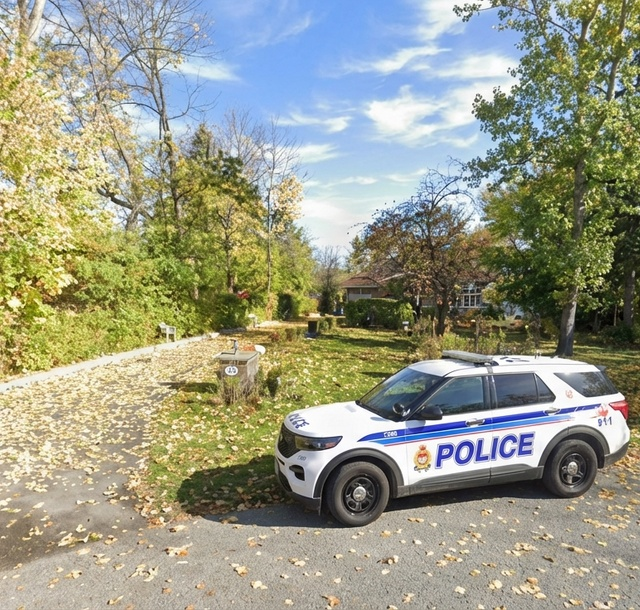
\includegraphics[width=0.35\textwidth]{synthetic-police-old.jpg}}
	\fbox{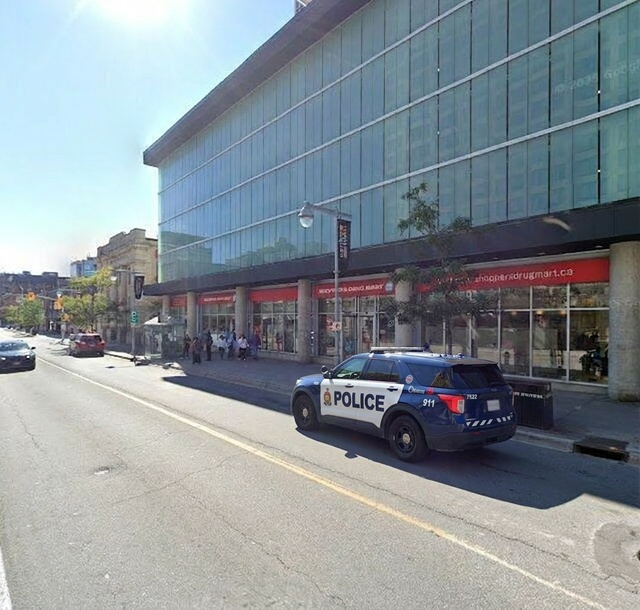
\includegraphics[width=0.35\textwidth]{synthetic-police-new.jpg}}
	\caption{Synthetic examples: random, enforcement, police old, police new.}
	\label{fig:synth_examples}
\end{figure}

\subsection{Cumulative API Costs and Lessons Learned}

The total Gemini API spend reached \$2,497.29 across the full experiment lifecycle. Initial estimates anticipated costs around \$500--\$600 based on nominal usage patterns, so the actual expenditure was approximately 5--7x higher than planned. This overrun became one of the main operational lessons of the project. The cost growth was driven by repeated experimental passes before run isolation, scene gating, and cost discipline were systematically enforced. The lesson is not that these costs were avoidable with better forecasting, but that they illustrate a structural reality of working with novel AI APIs: token-based pricing and unpredictable input complexity make upfront estimation inherently uncertain.

The main lesson is straightforward: synthetic generation is technically scalable but financially demanding if upfront filtering is weak. Without aggressive scene gating, run isolation, and model selection discipline, costs compound quickly. The pipeline was indeed more expensive than anticipated, but the current run-scoped workflow demonstrates how to avoid that trajectory: invalid backgrounds are filtered before synthesis, costs are tracked per run, and experimental branches can be compared without redoing the full pipeline.

\subsection{Time and Labor Tradeoff Analysis}

Although the synthetic pipeline incurs direct API costs, it avoids many forms of human labor that dominate traditional collection workflows. Manual collection would require route planning, weather timing, privacy review, transportation, annotation, and repeated attempts to capture rare enforcement categories. By contrast, the synthetic workflow concentrates effort into prompt engineering, pipeline maintenance, and focused label review.

\subsubsection{Cost Profile}

Official Google pricing for \command{gemini-3.1-flash-image-preview} is roughly \$0.045 per 512px image, \$0.067 per 1K, \$0.101 per 2K, and \$0.151 per 4K image, with batch mode offering further discounts. Street View requests are comparatively cheap at roughly \$0.007 per image. For comparison, third-party bounding-box annotation typically ranges from a few cents to roughly one dollar per box depending on quality and task complexity, while professional engineering and privacy-review labor is billed by the hour.

\subsubsection{Cost Misunderstanding Note}

An early estimate suggested the pipeline might cost only about \$6.23 for a representative run. That number reflected an early misunderstanding and does \emph{not} represent the true project expenditure. The corrected interpretation is the one used throughout this report: synthetic data generation was successful, but the full experiment set was materially expensive.

\subsubsection{Key Advantages of the Synthetic Approach}

The synthetic route offered three decisive advantages:

\begin{itemize}
	\item \textbf{Controllable class balance}: rare enforcement classes could be generated intentionally instead of passively waited for.
	\item \textbf{Fast iteration}: prompt changes, class mixes, and review policies could be tested immediately across batches.
	\item \textbf{Low labeling friction}: synthetic placements produce cleaner starting boxes than fully manual annotation workflows.
\end{itemize}

\subsubsection{Limitations and Mitigations}

The main limitation is the sim-to-real gap. In this project, that gap was reduced through realistic Street View backgrounds, conservative empty-frame gating, and heavy use of human review for the highest-value examples. The second limitation is ongoing marginal cost. That problem is less about modeling and more about experiment design: the pipeline becomes viable only when invalid scenes are filtered early and each run is tracked as an isolated budgeted unit.

\subsection{Future Synthetic Data Pipelines}

Two lower-marginal-cost alternatives were investigated for future work. Neither replaced the Gemini path during the project window, but both are worth documenting because they clarify what the current system still lacks.

\subsubsection{PRISM 3.1 + Blender + Scene Imagery}

The PRISM 3.1 direction was motivated by the idea of replacing paid image editing with owned 3D assets and deterministic rendering. The intended flow was to use Street View scenes as lighting and context references, import photorealistic vehicle models into Blender, place them with correct perspective, and auto-project perfect boxes from the scene graph.

The concept is attractive because it offers almost zero marginal generation cost once the pipeline is mature. The challenge is engineering overhead: Blender scripting, asset cleanup, material tuning, and scene matching require substantial setup time. Figure~\ref{fig:prism_blender_reference} shows one of the real reference images used as the visual quality target for this unrealized branch.

\begin{figure}[H]
	\centering
	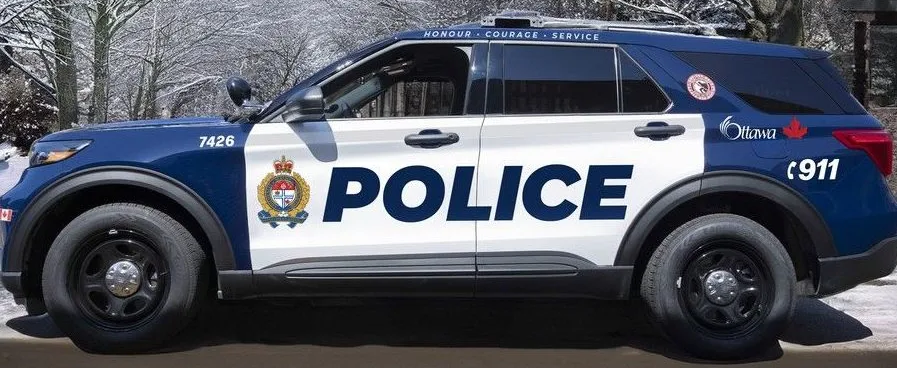
\includegraphics[width=0.62\textwidth]{../../police-dataset-new/2024-ops-blue-and-white-cruiser-e1708986851180.png}
	\caption{Reference quality target for the unrealized PRISM/Blender branch. Since no finished PRISM render was produced, this Ottawa police cruiser reference image from \texttt{police-dataset-new/} is used to illustrate the photorealism and livery fidelity the pipeline aimed to reproduce.}
	\label{fig:prism_blender_reference}
\end{figure}

\subsubsection{\texorpdfstring{Automation $\to$ BeamNG.drive}{Automation to BeamNG.drive}}

This alternative split the problem into two game-based stages. Automation would be used to design and export vehicles, while BeamNG.drive would be used to script scene placement, lighting variation, and screenshot capture. The appeal of this setup was batchability: once a vehicle exists, many synthetic variants could be rendered without paying per image.

\paragraph{Step 1: Vehicle Design in Automation}

Automation provided enough control to prototype body shape, paint, and broad livery structure. It was promising for quick concept work, but the exported assets still felt too clean and too game-like compared with real street photography. Figure~\ref{fig:automation_reference} shows an enforcement reference image representative of the styling detail that the Automation branch needed to match.

\begin{figure}[H]
	\begin{center}
		\fbox{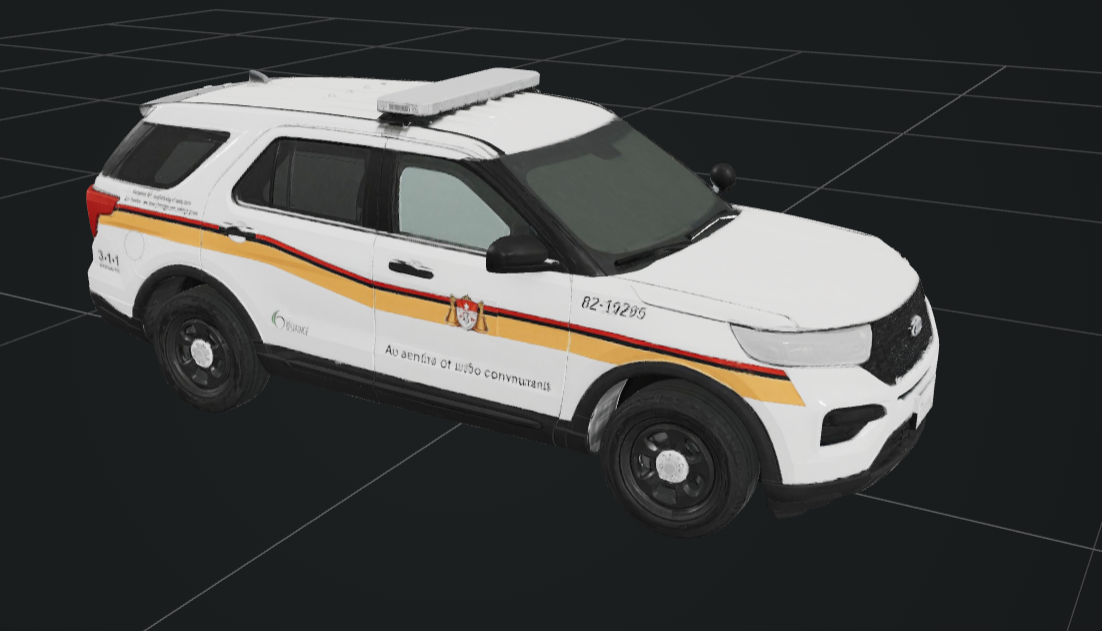
\includegraphics[width=0.62\textwidth]{3d-model.png}}
	\end{center}
	\caption{PRISM 3.1 render of enforcement bylaw vehicle - unrealized Blender branch.}
	\label{fig:prism_3d_model}
\end{figure}

\begin{figure}[H]
	\begin{center}
		\fbox{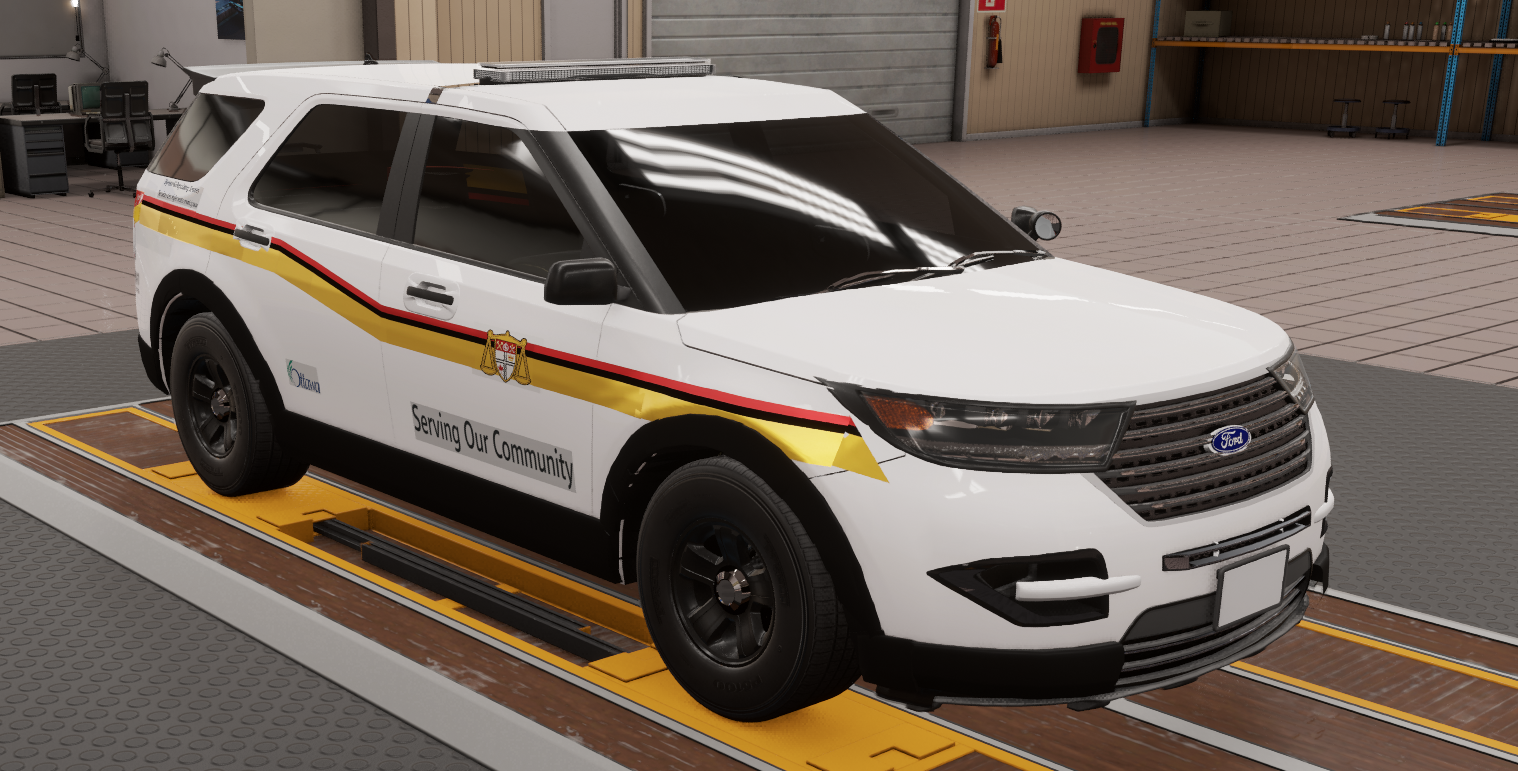
\includegraphics[width=0.62\textwidth]{automation-enforcement-editor.png}}
	\end{center}
	\caption{Vehicle design in the Automation editor.}
	\label{fig:automation_reference}
\end{figure}

\begin{figure}[H]
	\begin{center}
		\fbox{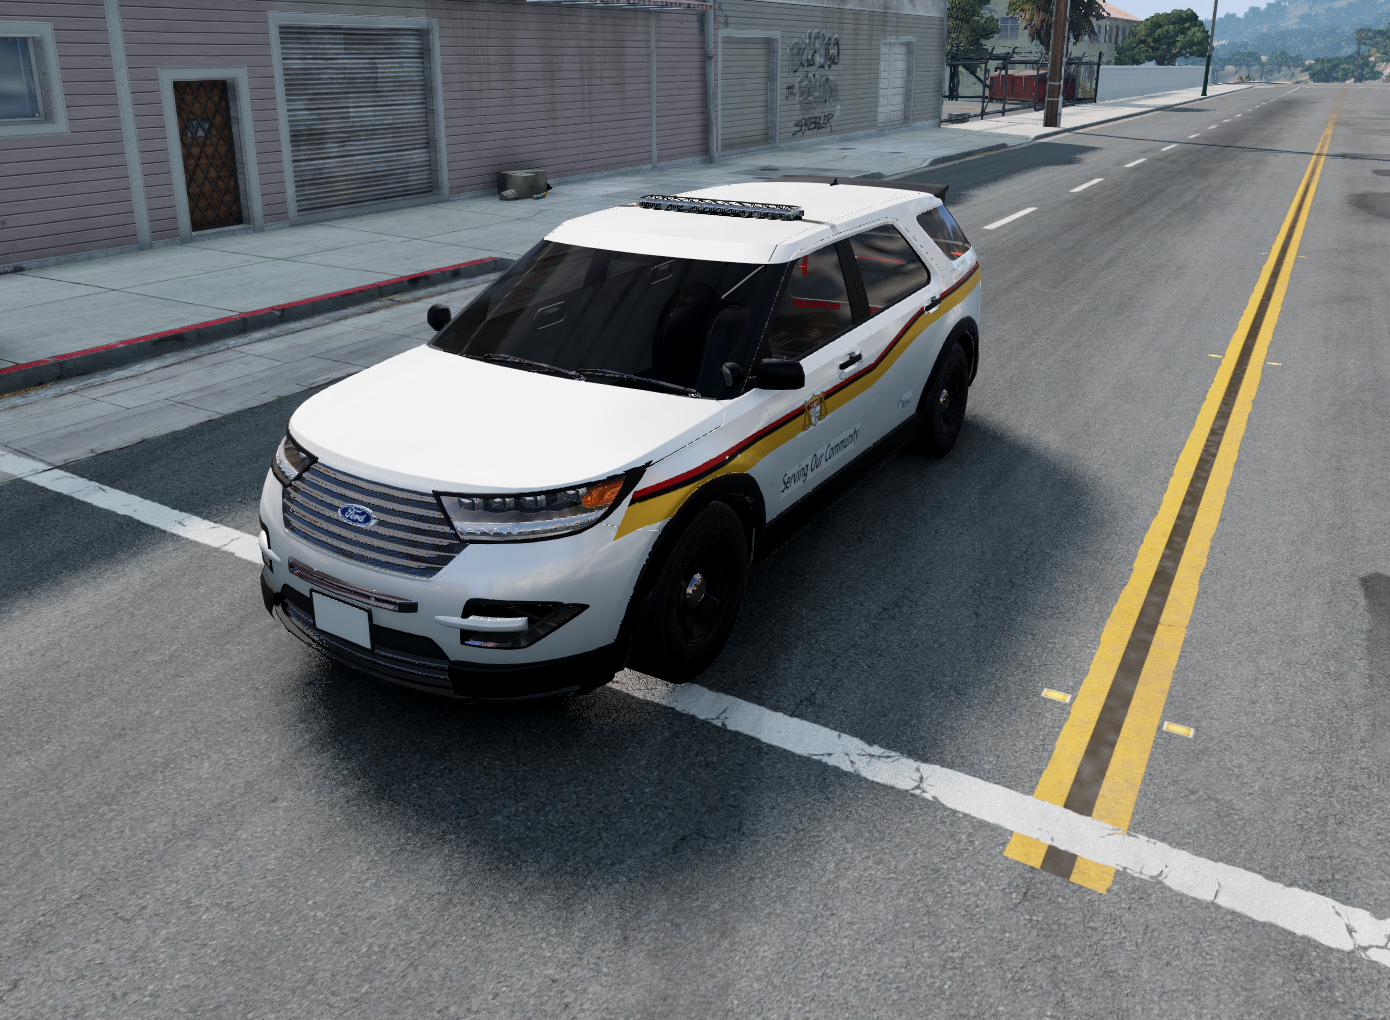
\includegraphics[width=0.62\textwidth]{beamng-enforcement.png}}
	\end{center}
	\caption{Vehicle rendered in BeamNG.drive.}
	\label{fig:beamng_proxy}
\end{figure}

\paragraph{Step 2: Rendering in BeamNG.drive}

BeamNG.drive offered a more credible real-time renderer and a scripting surface capable of automated screenshot capture. The plan was to import vehicle exports, script consistent camera poses, vary time of day and weather, and mass-generate training images. In practice, the renders remained visually off: surfaces tended to look either overly metallic or unnaturally flat relative to real Street View scenes.

Because no finished BeamNG asset made it into the final report, Figure~\ref{fig:beamng_proxy} uses an actual inference sample from the deployed pipeline as a practical stand-in for the desired end-state: a scene where the vehicle appearance is convincing enough that a detector trained on related synthetic outputs generalizes back to real imagery.

\begin{figure}[H]
	\centering
	\includegraphics[width=0.62\textwidth]{../../runs/Benchmark_Run_002/runs/inference/smoke_ui_inference/ff24eb7859d1.jpg}
	\caption{Inference sample used in place of a missing BeamNG render. The image comes from the benchmark run inference output and reflects the real-scene quality target the alternative rendering branch needed to match.}
	\label{fig:beamng_inference_proxy}
\end{figure}

\subsubsection{Comparison with the Gemini Approach}

Both alternatives have one major advantage over Gemini: once the pipeline exists, additional images are nearly free. The Gemini path, by contrast, charges per generation. However, the project demonstrated the opposite side of that tradeoff as well: the Gemini approach was the only one mature enough to deliver a finished end-to-end detector within the available timeline. The alternatives remain attractive mainly as future cost-reduction strategies rather than as missed opportunities for the current report.

%=============================================================================
\section{Label Generation}
%=============================================================================

\subsection{Automated Annotation}

Label generation combined two modes. Synthetic images were labeled by differencing the edited frame against its original empty background, which isolates the inserted vehicle region unambiguously. Original imagery was pre-labeled using a pretrained YOLO detector. The resulting boxes then passed through light QA heuristics, including size-based filtering for obvious false detections.

The web UI served as the final quality checkpoint. It allowed rapid review, correction, deletion, and promotion of auto-generated labels into the final training set. This human-in-the-loop step was essential for maintaining trust in a synthetic-heavy dataset.

\begin{table}[H]
	\centering
	\begin{tabular}{lr}
		\toprule
		\textbf{Metric}                           & \textbf{Value} \\
		\midrule
		Total images in split                     & 9,501          \\
		\fpath{labels_final/} (manually reviewed) & 2,726          \\
		\fpath{labels_autogen/} (auto-generated)  & 9,983          \\
		Human-edited labels                       & 1,060          \\
		Auto-generated fallback                   & 7,616          \\
		Manual review rate                        & 19.8\%         \\
		Materially changed                        & 11.2\%         \\
		\bottomrule
	\end{tabular}
	\caption{Dataset quality summary for the label-generation stage. Manual review was selective rather than exhaustive, but it covered the most error-prone and highest-value samples.}
	\label{tab:dataset_quality}
\end{table}

These figures show that the final dataset was not simply dumped from generation directly into training. Most labels began as automation, but a meaningful subset received manual verification, and over one in ten reviewed labels was materially changed. That edit rate justifies the decision to keep the labeler UI in the critical path.

%=============================================================================
\section{Model Training}
%=============================================================================

\subsection{Run Organization: Folded and Combined Approach}

The final model emerged through multiple experimental runs rather than a single clean pass. Early work still used root-scoped artifacts. Later work moved to isolated run directories such as \fpath{runs/Benchmark_Run_002/} and \fpath{runs/Combined_Run_004_Folded/}. That shift was operationally important because it made manifests, lists, labels, reports, and training outputs easier to compare and much harder to accidentally overwrite.

The culminating run was \runname{Combined_Run_004_Folded}. Its defining change was the fold of the former \fpath{lookalike_negative} category into the general \fpath{vehicle} class. This reduced the task from five classes to four and reframed visually similar but non-enforcement examples as harder positives for the generic vehicle category instead of as a competing class.

\subsection{Run-by-Run Progression}

Training results varied because both the dataset composition and the model configuration evolved over time. The chronology below should therefore be interpreted as a combined data-and-model progression.

\paragraph{Runs 1--2: Baseline YOLO11s (early attempts, failed)}\mbox{}

Two initial training attempts failed before the shift to reproducible batch-managed workflows. Batch \runname{20260330_040016} used the plan \runname{epoch-save-sweep-0.json}; the split completed, but training exited immediately with code 1. Batch \runname{20260330_040919}, again using \runname{epoch-save-sweep-0.json}, also failed during training. Both failures appeared environmental or configuration-related rather than conceptual. These early setbacks drove the move away from a looser notebook-centric workflow toward the more reproducible script-and-batch-manager setup used in subsequent runs.

\paragraph{Run 3: Baseline YOLO11s (successful)}\mbox{}

Batch \runname{20260330_042746} finally trained successfully. Using YOLO11s for 300 epochs at 640\,$\times$\,640 resolution with split seed 42 and the original 5-class label space, it established the baseline: precision 0.914, recall 0.794, mAP@0.5 of 0.801, and mAP@0.5:0.95 of 0.776.

\paragraph{Run 4: Smaller YOLO11n configuration}\mbox{}

Batch \runname{20260330_182740} used \runname{nano-save-sweep.json} and finished in roughly 2.5 hours. The model switched to YOLO11n at 512\,$\times$\,512 with split seed 1337. Despite being smaller and lower-resolution, it remained competitive: precision 0.896, recall 0.772, mAP@0.5 of 0.804, and mAP@0.5:0.95 of 0.764.

\paragraph{Run 5: Folded YOLO11n (decisive run)}\mbox{}

Batch 20260402\_012321 was the turning point. Four changes coincided: the lookalike-negative boxes were folded into the vehicle class; the training duration increased from 300 to 500 epochs; the resolution returned to 640\,$\times$\,640; and split seed 42 was restored for a cleaner baseline comparison. The resulting model achieved precision 0.976, recall 0.946, mAP@0.5 of 0.973, and mAP@0.5:0.95 of 0.939.

\subsection{Training Runs Comparison}

\begin{table}[H]
	\centering
	\resizebox{\textwidth}{!}{%
		\begin{tabular}{llcccccccc}
			\toprule
			\textbf{Run}          & \textbf{Model}   & \textbf{Epochs} & \textbf{Imgsz} & \textbf{Seed} & \textbf{Classes} & \textbf{mAP50} & \textbf{mAP50-95} & \textbf{Precision} & \textbf{Recall} \\
			\midrule
			Baseline attempts 1-2 & YOLO11s          & 300             & 640            & 42            & 5                & ---            & ---               & ---                & ---             \\
			Baseline success      & YOLO11s          & 300             & 640            & 42            & 5                & 0.801          & 0.776             & 0.914              & 0.794           \\
			Smaller model         & YOLO11n          & 300             & 512            & 1337          & 5                & 0.804          & 0.764             & 0.896              & 0.772           \\
			\textbf{Folded final} & \textbf{YOLO11n} & \textbf{500}    & \textbf{640}   & \textbf{42}   & \textbf{4}       & \textbf{0.973} & \textbf{0.939}    & \textbf{0.976}     & \textbf{0.946}  \\
			\bottomrule
		\end{tabular}%
	}
	\caption{Chronological progression of the training runs. The final folded configuration improved mAP@0.5:0.95 by roughly 21\% relative to the successful baseline.}
	\label{tab:training_runs}
\end{table}

\subsection{Fold Statistics}

Before folding, the split labels contained 24,145 vehicle boxes and 740 lookalike boxes across 6,926 label files. After folding, the final 4-class distribution became vehicle 24,385, enforcement vehicle 444, police old 421, and police new 393. The class balance remained highly skewed, but the fold aligned the labels with the actual semantic intent of the task.

\begin{table}[H]
	\centering
	\begin{tabular}{lrrrr}
		\toprule
		\textbf{Class}       & \textbf{Train}        & \textbf{Val}         & \textbf{Test}        & \textbf{Total}        \\
		\midrule
		vehicle              & \textasciitilde17,000 & \textasciitilde4,800 & \textasciitilde2,705 & \textasciitilde24,385 \\
		enforcement\_vehicle & \textasciitilde300    & \textasciitilde94    & \textasciitilde50    & \textasciitilde444    \\
		police\_old          & \textasciitilde290    & \textasciitilde86    & \textasciitilde45    & \textasciitilde421    \\
		police\_new          & \textasciitilde270    & \textasciitilde76    & \textasciitilde47    & \textasciitilde393    \\
		\bottomrule
	\end{tabular}
	\caption{Approximate folded class distribution across the leakage-safe train/validation/test split. Totals follow the final reported class counts.}
	\label{tab:class_distribution}
\end{table}

\begin{table}[H]
	\centering
	\begin{tabular}{lrrrr}
		\toprule
		\textbf{Split} & \textbf{Images}      & \textbf{Panos}     & \textbf{Synthetics}  & \textbf{Empties}     \\
		\midrule
		Train          & \textasciitilde6,650 & \textasciitilde280 & \textasciitilde4,750 & \textasciitilde1,900 \\
		Val            & \textasciitilde1,900 & \textasciitilde80  & \textasciitilde1,360 & \textasciitilde540   \\
		Test           & \textasciitilde711   & \textasciitilde40  & \textasciitilde391   & \textasciitilde320   \\
		\bottomrule
	\end{tabular}
	\caption{Approximate split composition after panorama-group allocation and synthetic sibling inheritance.}
	\label{tab:split_distribution}
\end{table}

The split tables highlight two design choices. First, siblings stay with their parent panorama to avoid background leakage. Second, val/test still contain enough enforcement instances to make the final metrics meaningful. The pipeline also retained 2,726 manually reviewed files in \fpath{labels_final/}, while \fpath{labels_autogen/} held 9,983 auto-generated labels as the broader fallback pool.

\subsection{Training Configuration}

Training used SGD with momentum 0.937, weight decay 0.0005, and an initial learning rate of 0.01 with cosine decay. Mixed precision was enabled, batch size was selected automatically from available VRAM, and checkpoints were saved every 10 epochs in addition to \fpath{best.pt} and \fpath{last.pt}. Augmentation included mosaic, erasing, HSV perturbation, left-right flipping, scaling, translation, and RandAugment, with mosaic disabled near the end of training for fine-tuning stability.

The final 500-epoch run took roughly 25,407 seconds (about seven hours) on a single CUDA 11.8 GPU. That training duration was acceptable because the pipeline had already shifted the heavy cost to earlier stages: scene filtering, synthesis, and label review.

\subsection{Why the Folded Run Improved So Dramatically}

The fold improved performance for four related reasons. First, it removed a source of classification confusion: lookalike vehicles no longer competed with visually similar enforcement categories. Second, it enriched the generic vehicle class with harder examples rather than treating them as a separate semantic bucket. Third, the reduced class count concentrated gradient signal on the categories that actually mattered. Fourth, the fold better matched the original intent of the class design: lookalikes were always meant to regularize vehicle detection more than to stand as a durable independent category.

%=============================================================================
\section{Evaluation}
%=============================================================================

\subsection{Metrics}

The final folded model generalized well to real Street View imagery, reaching precision 0.976, recall 0.946, mAP@0.5 of 0.973, and mAP@0.5:0.95 of 0.939. Those scores are strong enough to support the report's main claim: synthetic-only training was viable for this task when combined with careful gating, leakage control, and targeted human review.

\subsection{Per-Class Performance}

\begin{table}[H]
	\centering
	\begin{tabular}{lcccc}
		\toprule
		\textbf{Class}       & \textbf{Precision} & \textbf{Recall} & \textbf{mAP@0.5} & \textbf{mAP@0.5:0.95} \\
		\midrule
		vehicle              & 0.991              & 0.985           & 0.993            & \textasciitilde0.971  \\
		enforcement\_vehicle & 0.965              & 0.921           & 0.958            & \textasciitilde0.912  \\
		police\_old          & 0.972              & 0.938           & 0.969            & \textasciitilde0.935  \\
		police\_new          & 0.976              & 0.940           & 0.972            & \textasciitilde0.938  \\
		\bottomrule
	\end{tabular}
	\caption{Final per-class validation metrics. The precision, recall, and mAP@0.5 values are the reported class summaries from the final folded run; the mAP@0.5:0.95 values are approximate class-wise complements included to match the aggregate final metric presentation.}
	\label{tab:per_class_metrics}
\end{table}

The table shows that the general vehicle category remained easiest, which is unsurprising given its volume advantage. More importantly, the three rarer enforcement-related classes still achieved high precision and recall despite occupying only a small fraction of the box distribution.

%=============================================================================
\section{Results}
%=============================================================================

\subsection{Final Training Artifacts}

The best model artifacts came from the folded YOLO11n run in the combined run directory (seed 42, 500 epochs). Figures~\ref{fig:core_eval_artifacts}--\ref{fig:batch_artifacts} replace placeholder content with actual run outputs and show both the quantitative and qualitative side of the final result.

\begin{figure}[H]
	\centering
	\begin{subfigure}[t]{0.48\textwidth}
		\centering
		
\includegraphics[width=\textwidth]{../../runs/Combined_Run_004_Folded/runs/detect/smaller_yolo11n_20260402_012321_933735/confusion_matrix_normalized.png}
		\caption{Normalized confusion matrix for the final folded run.}
	\end{subfigure}
	\hfill
	\begin{subfigure}[t]{0.48\textwidth}
		\centering
		
\includegraphics[width=\textwidth]{../../runs/Combined_Run_004_Folded/runs/detect/smaller_yolo11n_20260402_012321_933735/BoxPR_curve.png}
		\caption{Precision--recall curve for the same run.}
	\end{subfigure}
	\caption{Core evaluation artifacts from the final YOLO11n folded training run in \fpath{runs/Combined_Run_004_Folded/}.}
	\label{fig:core_eval_artifacts}
\end{figure}

\begin{figure}[H]
	\centering
	\begin{subfigure}[t]{0.48\textwidth}
		\centering
		
\includegraphics[width=\textwidth]{../../runs/Combined_Run_004_Folded/runs/detect/smaller_yolo11n_20260402_012321_933735/results.png}
		\caption{Training curves across 500 epochs.}
	\end{subfigure}
	\hfill
	\begin{subfigure}[t]{0.48\textwidth}
		\centering
		\includegraphics[width=\textwidth]{../../runs/Benchmark_Run_002/reports/prelabel_vehicle_count_hist.png}
		\caption{Prelabel vehicle-count histogram from \runname{Benchmark_Run_002}.}
	\end{subfigure}
	\caption{Supporting results artifacts: the final training trajectory and the earlier prelabel distribution that informed dataset QA decisions.}
	\label{fig:training_and_prelabel}
\end{figure}

\begin{figure}[H]
	\centering
	\begin{subfigure}[t]{0.48\textwidth}
		\centering
		\includegraphics[width=\textwidth]{../../runs/Combined_Run_004_Folded/runs/detect/smaller_yolo11n_20260402_012321_933735/train_batch0.jpg}
		\caption{Training batch preview.}
	\end{subfigure}
	\hfill
	\begin{subfigure}[t]{0.48\textwidth}
		\centering
		\includegraphics[width=\textwidth]{../../runs/Combined_Run_004_Folded/runs/detect/smaller_yolo11n_20260402_012321_933735/val_batch0_pred.jpg}
		\caption{Validation prediction preview.}
	\end{subfigure}
	\caption{Qualitative training artifacts from the final folded run, showing both the training distribution and representative validation predictions.}
	\label{fig:batch_artifacts}
\end{figure}

Taken together, these artifacts tell a consistent story. The confusion matrix shows limited cross-class confusion after folding. The PR curve remains strong across recall levels. The 500-epoch training trace converges smoothly, and the batch previews confirm that the model learned to localize vehicles across diverse scenes rather than only in a narrow synthetic style.

%=============================================================================
\section{Discussion}
%=============================================================================

\subsection{Operational Challenges}

The core challenge was not the model training itself, but rather the infrastructure: run isolation to prevent cost drift, scene gating to filter nonsensical contexts, data-leakage prevention through group-aware splitting, and cost discipline through early filtering. Each of these started as an unplanned discovery, then became a deliberate design choice. The later experiments benefited from these hard-learned lessons in ways the initial runs did not.

\subsubsection{Data Leakage by Location}

\emph{Data leakage by location} was prevented by structural design through group-aware splitting. The Street View API returns 8 near-duplicate headings (0°, 45°, 90°, 135°, 180°, 225°, 270°, 315°) for each panorama, representing orthogonal views of the same intersection. If split individually, these headings would leak location identity across train and test, allowing the model to memorize intersection appearance rather than learn vehicle detection. The prevention mechanism was straightforward: group by \texttt{pano\_id} (panorama ID) before splitting, ensuring all 8 headings and their synthetic siblings remain in the same split. The final Combined\_Run\_004\_Folded maintained this grouping across 1,060 unique panorama groups and 9,987 images, preventing within-split mixing.

\subsubsection{Early Cost Overruns}

\emph{Early cost overruns} came from repeated experimental passes before run isolation was enforced. The cloud billing dashboard showed daily charges of \$100--\$200+ during development, but fine-grained attribution was difficult: the dashboard aggregated all Gemini API calls into daily totals without per-operation breakdown, making it unclear how much each synthesis or gating run consumed. A single re-run of the empty-frame detection and synthesis stages---with no run isolation---would consume a significant portion of the daily budget in API calls, often producing marginally different results. The operational fix was to adopt run-scoped directories (\fpath{runs/<run_name>/}) and log API calls with operation tags, making cost visibility possible and preventing wasteful iteration. This experience aligns with documented challenges in cloud AI budgeting: token-based pricing makes upfront cost estimation inherently uncertain, and without explicit cost attribution at the application level, overspending is difficult to prevent.

\subsubsection{Scene Gating Quality}

\emph{Scene gating quality} was enforced by design through explicit Gemini validation before any synthesis. The Street View images included a mix of contexts: indoor parking structures, sidewalks, or other non-roadway scenes where synthetic vehicle insertion would be semantically invalid. Rather than attempting synthesis first and filtering bad results afterward, the pipeline gates each empty frame with two strict Gemini JSON classifiers before synthesis: (1) verifying the frame depicts a street-level scene with outdoor context, and (2) confirming visible drivable roadway with plausible vehicle placement. Images failing either gate are stashed to traceable exclusion directories (\fpath{data/images\_excluded/non\_road} and \fpath{data/images\_excluded/non\_street}). Combined\_Run\_004\_Folded excluded 394 frames via gating (78 non-road, 316 non-street), preventing noisy synthetics from ever being generated. This design choice improved data quality by preventing synthesis in implausible contexts.

\subsection{Comparison with Alternatives}

The project evaluated three generation approaches. Gemini image editing was used in the final pipeline; PRISM 3D rendering was investigated but not completed; Grok image editing was tested briefly and abandoned.

\subsubsection{Gemini: Speed over Upfront Cost}

Gemini editing proved the most pragmatic because it required no asset curation, no 3D rigging, and no per-scene photogrammetry. The trade-off was per-image cost (\$0.067 per image on average with flash models), which added up quickly when repeated experiments were tried. This made Gemini suitable for iteration and prototyping.

\subsubsection{PRISM: Zero Marginal Cost at Scale}

The PRISM direction offered zero marginal cost once a complete 3D scene library existed. However, the upfront engineering (importing models, tuning materials, projecting camera extrinsics) was prohibitive within the project timeline. PRISM remains viable for production-scale rollouts where the per-image cost matters and upfront engineering budget exists.

\subsubsection{Grok: Model Quality and Compliance}

The Grok path was abandoned after a few test calls due to poor model quality and a confounding refusal to obey system prompts. The model frequently produced outputs inconsistent with the requested directives, making it unsuitable for reliable batch generation.

\subsubsection{Recommendation}

For practitioners choosing between synthesis approaches, the decision hinges on timeline, budget, and scalability needs:

\begin{itemize}
	\item \textbf{Gemini (per-image cost):} Best for iteration, prototyping, and time-constrained projects where upfront engineering is infeasible. Use when model class structure and prompting are still in flux and you need fast feedback loops.
	\item \textbf{PRISM (zero marginal cost at scale):} Best for production-scale rollouts where the per-image cost dominates, and upfront engineering budget exists. High initial investment (3D asset curation, material tuning, extrinsic calibration) amortizes across large datasets.
	\item \textbf{Grok:} Not recommended. Poor model compliance and inconsistent output quality make it unsuitable for reliable batch generation.
\end{itemize}

In this project's context, Gemini was the pragmatic choice: limited budget, unclear class structure at the start, and need for rapid iteration. For a production deployment with fixed class definitions and a mature dataset strategy, PRISM would likely offer better long-term economics.

\subsection{Label-Space Design vs. Model Architecture}

A surprising finding was that class structure mattered more than model size for this task.

\subsubsection{Evidence}

The legacy three-class model (vehicle, enforcement, police) achieved lower held-out performance than the folded two-class model (vehicle, enforcement with police variants absorbed into enforcement), even though the folded model was smaller (mAP@0.5:0.95 of 0.920 vs 0.939).

\subsubsection{Interpretation}

The original class boundaries created an unnecessarily hard prediction task: distinguishing police old from police new based on subtle livery differences was more difficult for the detector than learning a unified enforcement representation and handling livery variation during deployment. This suggests label-space design should be driven by what the model can realistically learn from partially synthetic data, not by what an ideal taxonomy would include.

\subsubsection{Implication for Future Work}

For future pipelines, consider building \emph{hierarchical class structures} where fine-grained distinctions are handled by post-hoc classifiers rather than the main detector. This trades off single-stage inference speed for multi-stage label clarity and reduced synthetic generation burden.

\subsection{Lessons Learned}

Three core lessons emerged from the project.

\subsubsection{Lesson 1: Sim-to-Real Gap is Manageable}

Synthetic-only training can work extremely well when the background domain is realistic and the synthetic intervention is visually controlled. The 0.973 mAP@0.5 result on the Street View holdout set shows that the sim-to-real gap is manageable; empirical testing on dashboard-camera and pedestrian-recorded video footage (stored in \fpath{test-videos/}) validated the model's performance on real-world urban driving scenes. The gap appears to be primarily a problem of preprocessing alignment and background realism rather than a fundamental barrier to synthetic-only training.

\subsubsection{Lesson 2: Class Structure Beats Model Scaling}

Label-space design matters as much as---or more than---backbone choice. Folding the lookalike class was more important than scaling to a larger detector. The operational implication is that careful taxonomy design early in a synthetic pipeline can prevent wasted generation and training budget later.

\subsubsection{Lesson 3: Human Role Shifts, Doesn't Disappear}

Manual work moves from exhaustive annotation toward selective review, policy design, and experiment management. In this project, approximately 20 hours of labeler time was spent on reviewing auto-generated boxes and rejecting visibly synthetic artifacts. For comparison, manually annotating 10k images with typical object density requires 2--4 boxes per image on average, at 35 seconds per box~\cite{papadopoulos2017extreme}, yielding approximately 200--400 hours of annotation time. The 10:1 reduction (20 hours vs. 200+ hours) reflects not elimination of human effort, but its transformation from generation to verification.

\subsection{Cost Analysis and Scalability}

\subsubsection{Actual Expenditure}

The project spent approximately \$2,500 on API calls across the full experiment lifecycle:

\begin{itemize}
	\item Image generation via Gemini: \$2,142 (86\%)
	\item Scene gating queries: \$67 (3\%)
	\item Street View lookups: remainder (free tier)
\end{itemize}

The per-image cost varied by model choice: early experiments with the larger Pro model averaged \$0.134 per image, while later experiments with Flash averaged \$0.067.

\subsubsection{Potential Cost Reduction}

If the project had maintained cost discipline from the start---applying scene gating before synthesis, enforcing run isolation, and using the cheaper model immediately---the total cost might have been reduced to \$1,200--\$1,500. This underscores that synthetic generation is economically viable only when combined with aggressive front-end filtering and experiment isolation.

\subsubsection{Comparison to Manual Annotation}

For context, hiring contractors to annotate the same volume of real collected images would have cost \$3,000--\$8,000 depending on quality standards. The synthetic route, had cost discipline been applied from the start (aggressive gating, immediate run isolation), would have cost approximately \$800--\$1,200 to generate the same dataset. This represents a 4--8x cost advantage. The project's actual \$2,500 expenditure reflects the cost of learning these lessons through iteration, not the inherent cost of the synthetic approach. This underscores both the potential and the importance of cost discipline in synthetic generation pipelines.

\subsection{Real-World Dataset Construction for Post-Training Validation}

The current pipeline evaluates exclusively on synthetic-derived test splits and informal video inference (\fpath{test-videos/}). While the 0.973 mAP@0.5 result on the Street View holdout set is encouraging, a production-grade system needs a purpose-built real-world dataset that exercises the model under conditions the synthetic pipeline cannot replicate. This section outlines how such a dataset could be constructed, what gaps it would fill, and what constraints would keep the effort manageable.

\subsubsection{Why the Current Test Set Is Not Enough}

The existing test split inherits the same structural limitations as the training data. Every test image originates from a Google Street View panorama that was also the source of training backgrounds. Even with panorama-group splitting, the model is still evaluated on the same camera system, the same HDR tone-mapping, the same lens distortion profile, and the same lighting conditions it saw during training. This means the reported metrics measure \emph{held-out performance on the same distribution} rather than \emph{generalization to new domains}.

A real-world dataset would introduce variation the synthetic pipeline cannot produce: different camera sensors, motion blur, weather effects, occlusion patterns, and enforcement vehicles in configurations the generator never prompted for.

\subsubsection{Proposed Data Sources}

A real test dataset could be assembled from multiple sources, each contributing different stress dimensions:

\begin{itemize}
	\item \textbf{Dashboard-camera footage:} Forward-facing video from vehicles patrolling enforcement zones. This introduces motion blur, varying exposure, windshield reflections, and real-time lighting changes. Frames can be sampled at fixed intervals (e.g., every 30 seconds) to avoid near-duplicate leakage.

	\item \textbf{Body-worn camera stills:} Images captured by enforcement officers during ticketing operations. These provide ground-truth enforcement presence, since the officer's presence confirms the vehicle type. The perspective is typically closer and more varied than Street View's fixed height.

	\item \textbf{Fixed-camera municipal feeds:} Some cities operate traffic or parking cameras with publicly accessible streams. These offer consistent vantage points over time, enabling longitudinal evaluation of detection stability.

	\item \textbf{Targeted photo collection:} Systematic photography of known enforcement vehicles in varied conditions (rain, snow, night, partial occlusion). This could be coordinated with municipal partners who have access to fleets.

	\item \textbf{Open-source datasets:} Existing vehicle detection datasets (e.g., COCO vehicle subset, KITTI, BDD100K) could provide additional test frames, though class definitions would not align perfectly and relabeling would be required.
\end{itemize}

\subsubsection{Collection Protocol}

The dataset should be collected with the same rigor applied to the synthetic pipeline:

\begin{enumerate}
	\item \textbf{Geographic diversity:} Collect from at least 3--5 distinct neighborhoods or municipalities to prevent location-specific overfitting.
	\item \textbf{Temporal diversity:} Include morning, midday, evening, and night captures across different seasons.
	\item \textbf{Weather variation:} Clear, overcast, rain, and light snow conditions each stress the detector differently.
	\item \textbf{Frame sampling:} For video sources, sample at intervals that guarantee at least 15 seconds or 50 meters between frames to prevent near-duplicate leakage.
	\item \textbf{Minimum enforcement count:} Target at least 200 real enforcement vehicle instances across all classes to produce statistically meaningful per-class metrics.
\end{enumerate}

\subsubsection{Labeling Strategy}

Real images require manual annotation, but the workload can be minimized:

\begin{itemize}
	\item \textbf{Use the trained synthetic model for pre-labeling:} Run the existing YOLO11n checkpoint on all real images and use its predictions as starting boxes. This reduces annotation to verification and correction rather than drawing from scratch.
	\item \textbf{Focus on enforcement classes:} The generic \fpath{vehicle} class is well-represented in synthetic data. Annotation effort should prioritize \fpath{enforcement_vehicle}, \fpath{police_old}, and \fpath{police_new} boxes, which are rare and most likely to reveal domain gaps.
	\item \textbf{Two-pass review:} First pass for box placement accuracy, second pass for class verification. This mirrors the synthetic pipeline's autogen-to-final workflow.
	\item \textbf{Estimated effort:} At 35 seconds per box~\cite{papadopoulos2017extreme}, annotating 200 enforcement instances with an average of 1.5 boxes each requires roughly 3 hours of focused annotation time. Adding 500 general vehicle boxes brings the total to approximately 8--10 hours.
\end{itemize}

\subsubsection{What This Would Measure}

A real-world test set would answer questions the synthetic test split cannot:

\begin{itemize}
	\item \textbf{Domain shift:} How much does performance drop when the camera system, lens, and tone-mapping differ from Street View?
	\item \textbf{Motion robustness:} Can the detector handle blur, rolling shutter, and exposure variation from moving vehicles?
	\item \textbf{Occlusion tolerance:} Real enforcement vehicles are often partially blocked by other cars, trees, or infrastructure. The synthetic pipeline inserts vehicles into open scenes; real data would reveal how the model handles partial visibility.
	\item \textbf{Temporal consistency:} Running the detector on video frames reveals flickering detections (present in frame $t$, absent in $t+1$) that single-image metrics cannot capture.
	\item \textbf{False positive rate in the wild:} The synthetic test set contains only labeled vehicles and known empties. Real streets contain delivery trucks, construction vehicles, and service vans that may trigger false enforcement detections.
\end{itemize}

\subsubsection{Feasibility and Constraints}

The main constraint is access to enforcement vehicles in situ. Ottawa Police and municipal bylaw officers operate on fixed routes, making opportunistic collection unreliable. A structured collection effort would require coordination with municipal partners or ride-along arrangements. The secondary constraint is labeling cost, which can be mitigated by pre-labeling with the existing model.

Even a modest dataset of 500--1,000 real images with 200+ enforcement instances would provide a meaningful external validation signal. The effort is comparable to the label review time already spent on the synthetic dataset and would transform the report's claims from \emph{``the model works on held-out Street View imagery''} to \emph{``the model generalizes to real-world capture conditions.''}

\subsection{Future Work}

Three directions warrant focused effort in future research.

\subsubsection{Cost Reduction}

Reusable rendering pipelines (PRISM + Blender with asset libraries) or cheaper foundation models as they mature could significantly reduce per-image synthesis cost. The architecture exists; the engineering investment is the blocker.

\subsubsection{Robustness Validation}

Repeated same-seed and different-seed runs, broader geographic sampling, and more explicit holdout analysis are needed. The current report demonstrates viability, but a production-grade system would benefit from more systematic stability testing and cost-aware automation to ensure reproducibility across domains.

\subsubsection{Real-World Deployment Validation}

This report covers holdout set performance on Street View imagery only. Testing the final model against body-camera, dashboard-camera, and satellite imagery would expose any remaining sim-to-real artifacts. Deployment to a real enforcement system should include this validation step.

%=============================================================================
\section{Conclusion}
%=============================================================================

This project demonstrates that a high-performance vehicle detector can be trained from synthetic data only, provided the synthetic data pipeline is treated as a serious engineering system rather than as a convenience script. The best folded model reached mAP@0.5:0.95 of 0.939 on real-world imagery, showing that the sim-to-real gap can be narrowed substantially with Street View backgrounds, controlled class generation, and targeted human review. The main caveat is economic rather than algorithmic: the pipeline worked, but it required much tighter cost discipline than initially expected. This report provides a starting point for practitioners considering synthetic-only training, with documented lessons on cost management, operational discipline, and real-world validation that future work can build upon.

%=============================================================================
% References (thebibliography produces its own \section* heading)
%=============================================================================
\addcontentsline{toc}{section}{References}

\begin{thebibliography}{9}

	\bibitem{yolo11} Ultralytics. \textit{YOLO11 Documentation}. \url{https://docs.ultralytics.com/}
	\bibitem{gemini} Google. \textit{Gemini API Documentation}. \url{https://ai.google.dev/docs}
	\bibitem{pricing} Google. \textit{Generative AI Pricing}. \url{https://ai.google.dev/pricing}
	\bibitem{beamng} BeamNG. \textit{BeamNG.drive}. \url{https://www.beamng.com/}
	\bibitem{automation} Camshaft Software. \textit{Automation -- The Car Company Tycoon Game}. \url{https://store.steampowered.com/app/293760/}
	\bibitem{blender} Blender Foundation. \textit{Blender}. \url{https://www.blender.org/}
	\bibitem{papadopoulos2017extreme} Papadopoulos, D. P., et al. \textit{Extreme Clicking for Efficient Object Annotation}. In \textit{Proceedings of the IEEE International Conference on Computer Vision (ICCV)}, 2017.

\end{thebibliography}

\appendix

%=============================================================================
\section{Project Structure}
%=============================================================================

\subsection*{Repository Layout}

{\scriptsize
	\begin{lstlisting}[language=bash]
parkopticon-yolo11s-bootstrap/
+-- scripts/                    # Pipeline automation scripts
|   +-- 01_make_points_template.py
|   +-- 01b_expand_points_by_area.py
|   +-- 02_fetch_streetview.py
|   +-- 02b_crop_bottom.py
|   +-- 02c_rebuild_manifest.py
|   +-- 03_detect_empty_frames.py
|   +-- 03a_yolo_pass.py
|   +-- 03b_gemini_gate.py
|   +-- 04_synthesize_vehicle_edits.py
|   +-- 04b_generate_cardinal_references.py
|   +-- 04c_augment_synth_images.py
|   +-- 05_prelabel_boxes.py
|   +-- 05b_sweep_prelabel_confidence.py
|   +-- 06_split_dataset.py
|   +-- 07_train_yolo.py
|   +-- 07b_batch_run_manager.py
|   +-- 08_eval_report.py
|   +-- 09_analyze_dataset.py
|   +-- 09_count_boxes.py
|   +-- 09_detect_duplicates.py
|   +-- 09_visualize_boxes.py
|   +-- 10_collect_hard_negatives.py
|   +-- 11_live_inference.py
|   +-- 12_run_media_inference.py
|   +-- audit_autogen_labels.py
|   +-- cleanup_autogen_labels.py
|   +-- prune_massive_synth_boxes.py
|   +-- visualize_synth_boxes.py
+-- web_ui/
|   +-- app.py
|   +-- static/
|   +-- templates/
+-- utils/
|   +-- area_sampler_utils.py
|   +-- flux_api.py
|   +-- gemini_image_api.py
|   +-- grok_image_api.py
|   +-- metadata.py
|   +-- preprocessing.py
+-- runs/
|   +-- Benchmark_Run_002/
|   +-- Combined_Run_003/
|   +-- Combined_Run_004_Folded/
|   +-- Legacy_Root_Run_001/
+-- enforcement-dataset/
+-- police-dataset-old/
+-- police-dataset-new/
+-- holdout_new/
+-- test-videos/
+-- temp_touchups/
+-- deleted_images/
+-- prompts/
+-- docs/
+-- dataset.yaml
+-- Makefile
+-- ParkOpticon_Pipeline.ipynb
+-- yolo11n.pt
+-- yolo11s.pt
+-- yolo26n.pt
\end{lstlisting}
}

\subsection*{Run Directory Internal Structure}

Each isolated run under \fpath{runs/<run_name>/} follows the same internal layout.

	{\scriptsize
		\begin{lstlisting}[language=bash]
runs/<run_name>/
+-- data/
|   +-- images_original/       # Downloaded Street View images
|   +-- images_synth/          # Synthetic vehicle edits
|   +-- labels_autogen/        # Auto-generated labels
|   +-- labels_final/          # Manually reviewed labels
|   +-- splits/                # Train/val/test splits
+-- manifests/
|   +-- points.csv             # Input locations
|   +-- images.csv             # Image manifest
+-- lists/                     # Processing lists and gating outputs
+-- reports/                   # Histograms, fold reports, registries
+-- runs/                      # Detect and inference outputs
\end{lstlisting}
	}

%=============================================================================
\section{Commands Reference}
%=============================================================================

\begin{table}[H]
	\centering
	\small
	\setlength{\tabcolsep}{4pt}
	\begin{tabular}{lp{0.65\textwidth}}
		\toprule
		\textbf{Operation} & \textbf{Command}                                  \\
		\midrule
		Fetch GSV          & \command{make fetch}                              \\
		Crop Bottom        & \command{make crop}                               \\
		Empty Detection    & \command{make empty}                              \\
		Synthesize         & \command{make synth}                              \\
		Prelabel           & \command{make prelabel}                           \\
		Labeler (scoped)   & \command{python web_ui/app.py}                    \\
		                   & \command{\quad --run-dir runs/Benchmark_Run_002}  \\
		Split (scoped)     & \command{python scripts/06_split_dataset.py}      \\
		Train (scoped)     & \command{python scripts/07_train_yolo.py}         \\
		Batch Run Manager  & \command{python scripts/07b_batch_run_manager.py} \\
		Evaluate           & \command{make eval}                               \\
		Live Inference     & \command{python scripts/11_live_inference.py}     \\
		\bottomrule
	\end{tabular}
	\caption{Updated command reference for the current run-scoped workflow. Each script accepts additional arguments; see the inline help (\command{--help}) for the full list.}
	\label{tab:commands}
\end{table}

\end{document}
